\documentclass{article}
\usepackage[utf8]{inputenc}
\usepackage[spanish]{babel}
\usepackage{graphicx}
\usepackage{listings}


\title{Informe Parcial II}
\author{daniel.perez19 }
\date{September 2021}

\begin{document}

\begin{titlepage}
    \begin{center}
        \vspace*{1cm}
            
        \Huge
        \textbf{Informe Parcial 2}
            
        \vspace{0.5cm}
        \LARGE
        Informática II
            
        \vspace{1.5cm}
            
        \textbf{Daniel Perez Gallego CC. 1193088770\\Jorge Montaña Cisneros CC.  1007327968}
            
        \vfill
            
        \vspace{0.8cm}
            
        \Large
        Departamento de Ingeniería Electrónica y Telecomunicaciones\\
        Universidad de Antioquia\\
        Medellín\\
        Septiembre de 2021
            
    \end{center}
\end{titlepage}

\tableofcontents
\vspace{2cm}
\section{Análisis}
\subsection{Análisis del problema}
Al analizar detenidamente el parcial y las instrucciones planteadas, observamos que el mayor reto consistiría en la modificación del tamaño de las imágenes, adaptándolo a un tamaño específico, ya sea aumentando o disminuyendo la proporción.\\ 

Para reducir el tamaño de la imagen, se hará un proceso de obtener bloques dividiendo el tamaño de las filas y columnas de la imagen actual por el tamaño deseado; estos bloques de pixeles serán promediados, obteniendo así un solo pixel RGB el cual representará la información en nuestra martiz deseada. En caso de que la división no sea entera, realizaremos un proceso de ajuste en el largo y/o ancho nuestra imagen.\\

Si la imagen dada tiene un tamaño menor al esperado, se hará un proceso de obtener bloques dividiendo el tamaño deseado por las filas y columnas de la imagen, esto nos dará el resultado de cuántas veces se multiplicarán los pixeles hasat quedar con la matriz deseada. En caso de que la división no sea entera, realizaremos un proceso de ajuste en el largo y/o ancho nuestra imagen. \\

Mientras más pequeña sea la matriz de LEDs, menos información deberemos exportar, será más eficiente y fácil, sin embargo, la imagen se volverá dificil de reconocer para el usuario.\\

\textbf{Submuestreo}\\
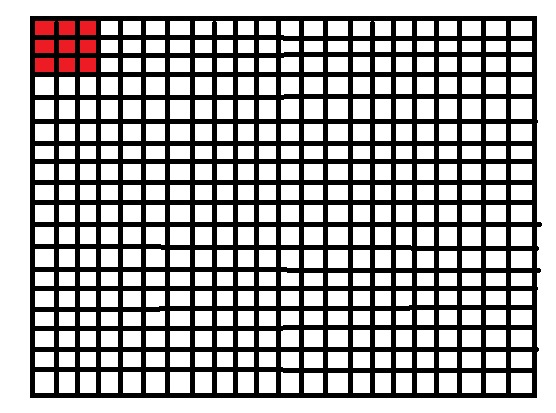
\includegraphics[width=6cm]{Imagenes/submuestreo.jpeg}\\
\textbf{Submuestreo}\\
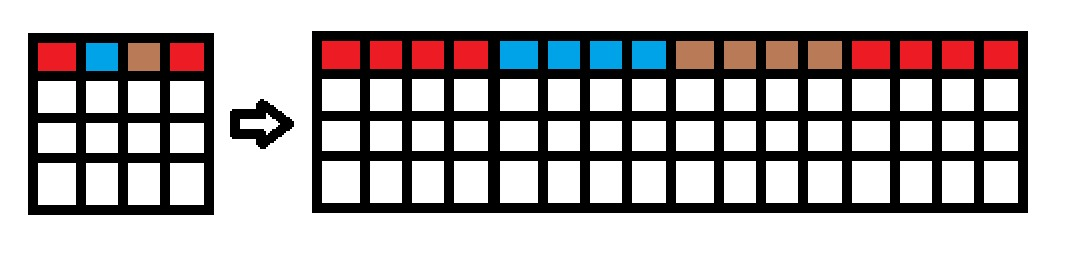
\includegraphics[width=6cm]{Imagenes/sobremuestreo.jpeg}\\

\vspace{0,3cm}

\subsection{Tareas a realizar}
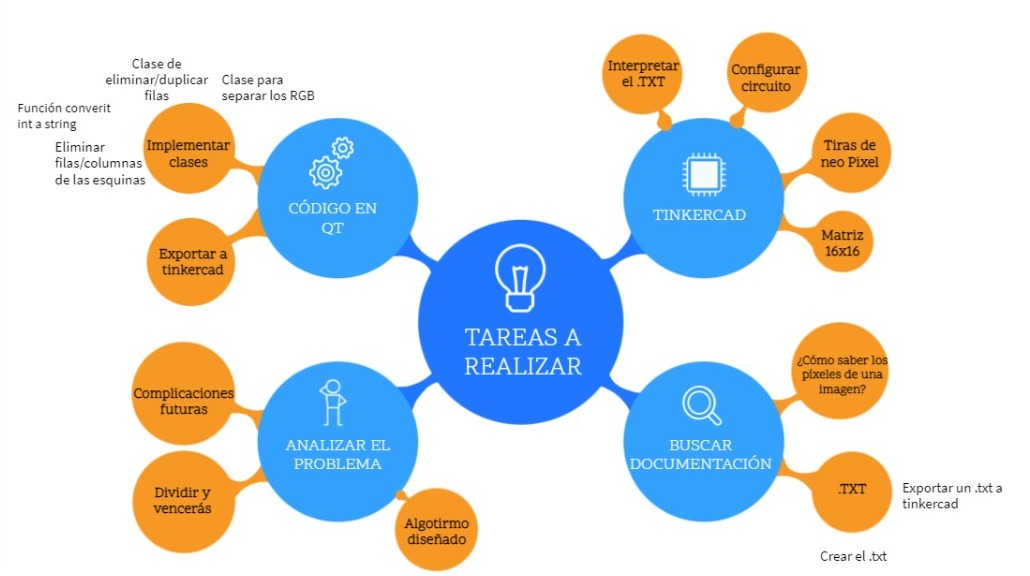
\includegraphics[width=15cm]{Imagenes/Esquema.jpeg}

\subsection{Algoritmo implementado}
Diagrama de flujo del algoritmo que implemenatremos para la solución del problema (No código)\\
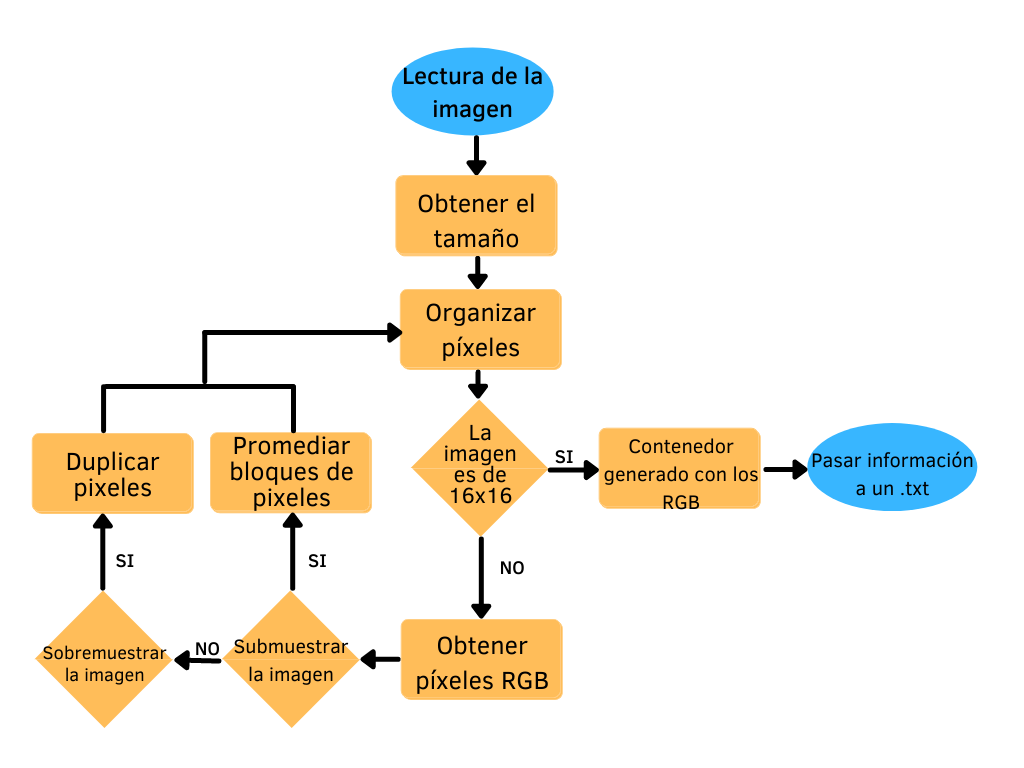
\includegraphics[width=14cm]{Imagenes/Diagrama.png}

\subsection{Consideraciones}
Una de las consideraciones más importantes que encontramos fué una correcta identificación de cada columna y fila de píxeles RGB, y mirar el modo de separar cada una.\\

El método y el formato para generar el .txt final y enviarlo a tinkercad.\\

Si una imagen tiene tamaños impares, como una que sea 101x113, se tendrán que realizar un proceso previo para evitar problemas\\

\end {document}
